% Gemini theme
% https://github.com/anishathalye/gemini

\documentclass[final,20pt]{beamer}

% ====================
% Packages
% ====================

\usepackage[ngerman]{babel}
\usepackage[T1]{fontenc}
\usepackage{lmodern}
\usepackage[size=a1,orientation=portrait,scale=1.4]{beamerposter}
\usetheme{gemini}
\usecolortheme{gemini}
\usepackage{graphicx}
\usepackage{tikz}
\usepackage{pgfplots}
\usepackage{svg}

% ====================
% Lengths
% ====================

% If you have N columns, choose \sepwidth and \colwidth such that
% (N+1)*\sepwidth + N*\colwidth = \paperwidth
\newlength{\sepwidth}
\newlength{\colwidth}
\setlength{\sepwidth}{0.02\paperwidth}
\setlength{\colwidth}{0.47\paperwidth}

\newcommand{\separatorcolumn}{\begin{column}{\sepwidth}\end{column}}
\addto\extrasngerman{\def\figureautorefname{Abb.}}
% ====================
% Title
% ====================

\title{Apoplexy - Ein Fitnesstracker zur Rehabilitation von Schlaganfall-Patienten}

\author{Lukas Rost}
\institute{Albert-Schweitzer-Gymnasium Erfurt}

% ====================
% Body
% ====================

\begin{document}

\begin{frame}[t]

\vspace{3cm}

\begin{columns}[t]
\separatorcolumn

\begin{column}{\colwidth}
   \begin{alertblock}{Hauptseite der App}
   	\begin{figure}[H]
   		\centering
   		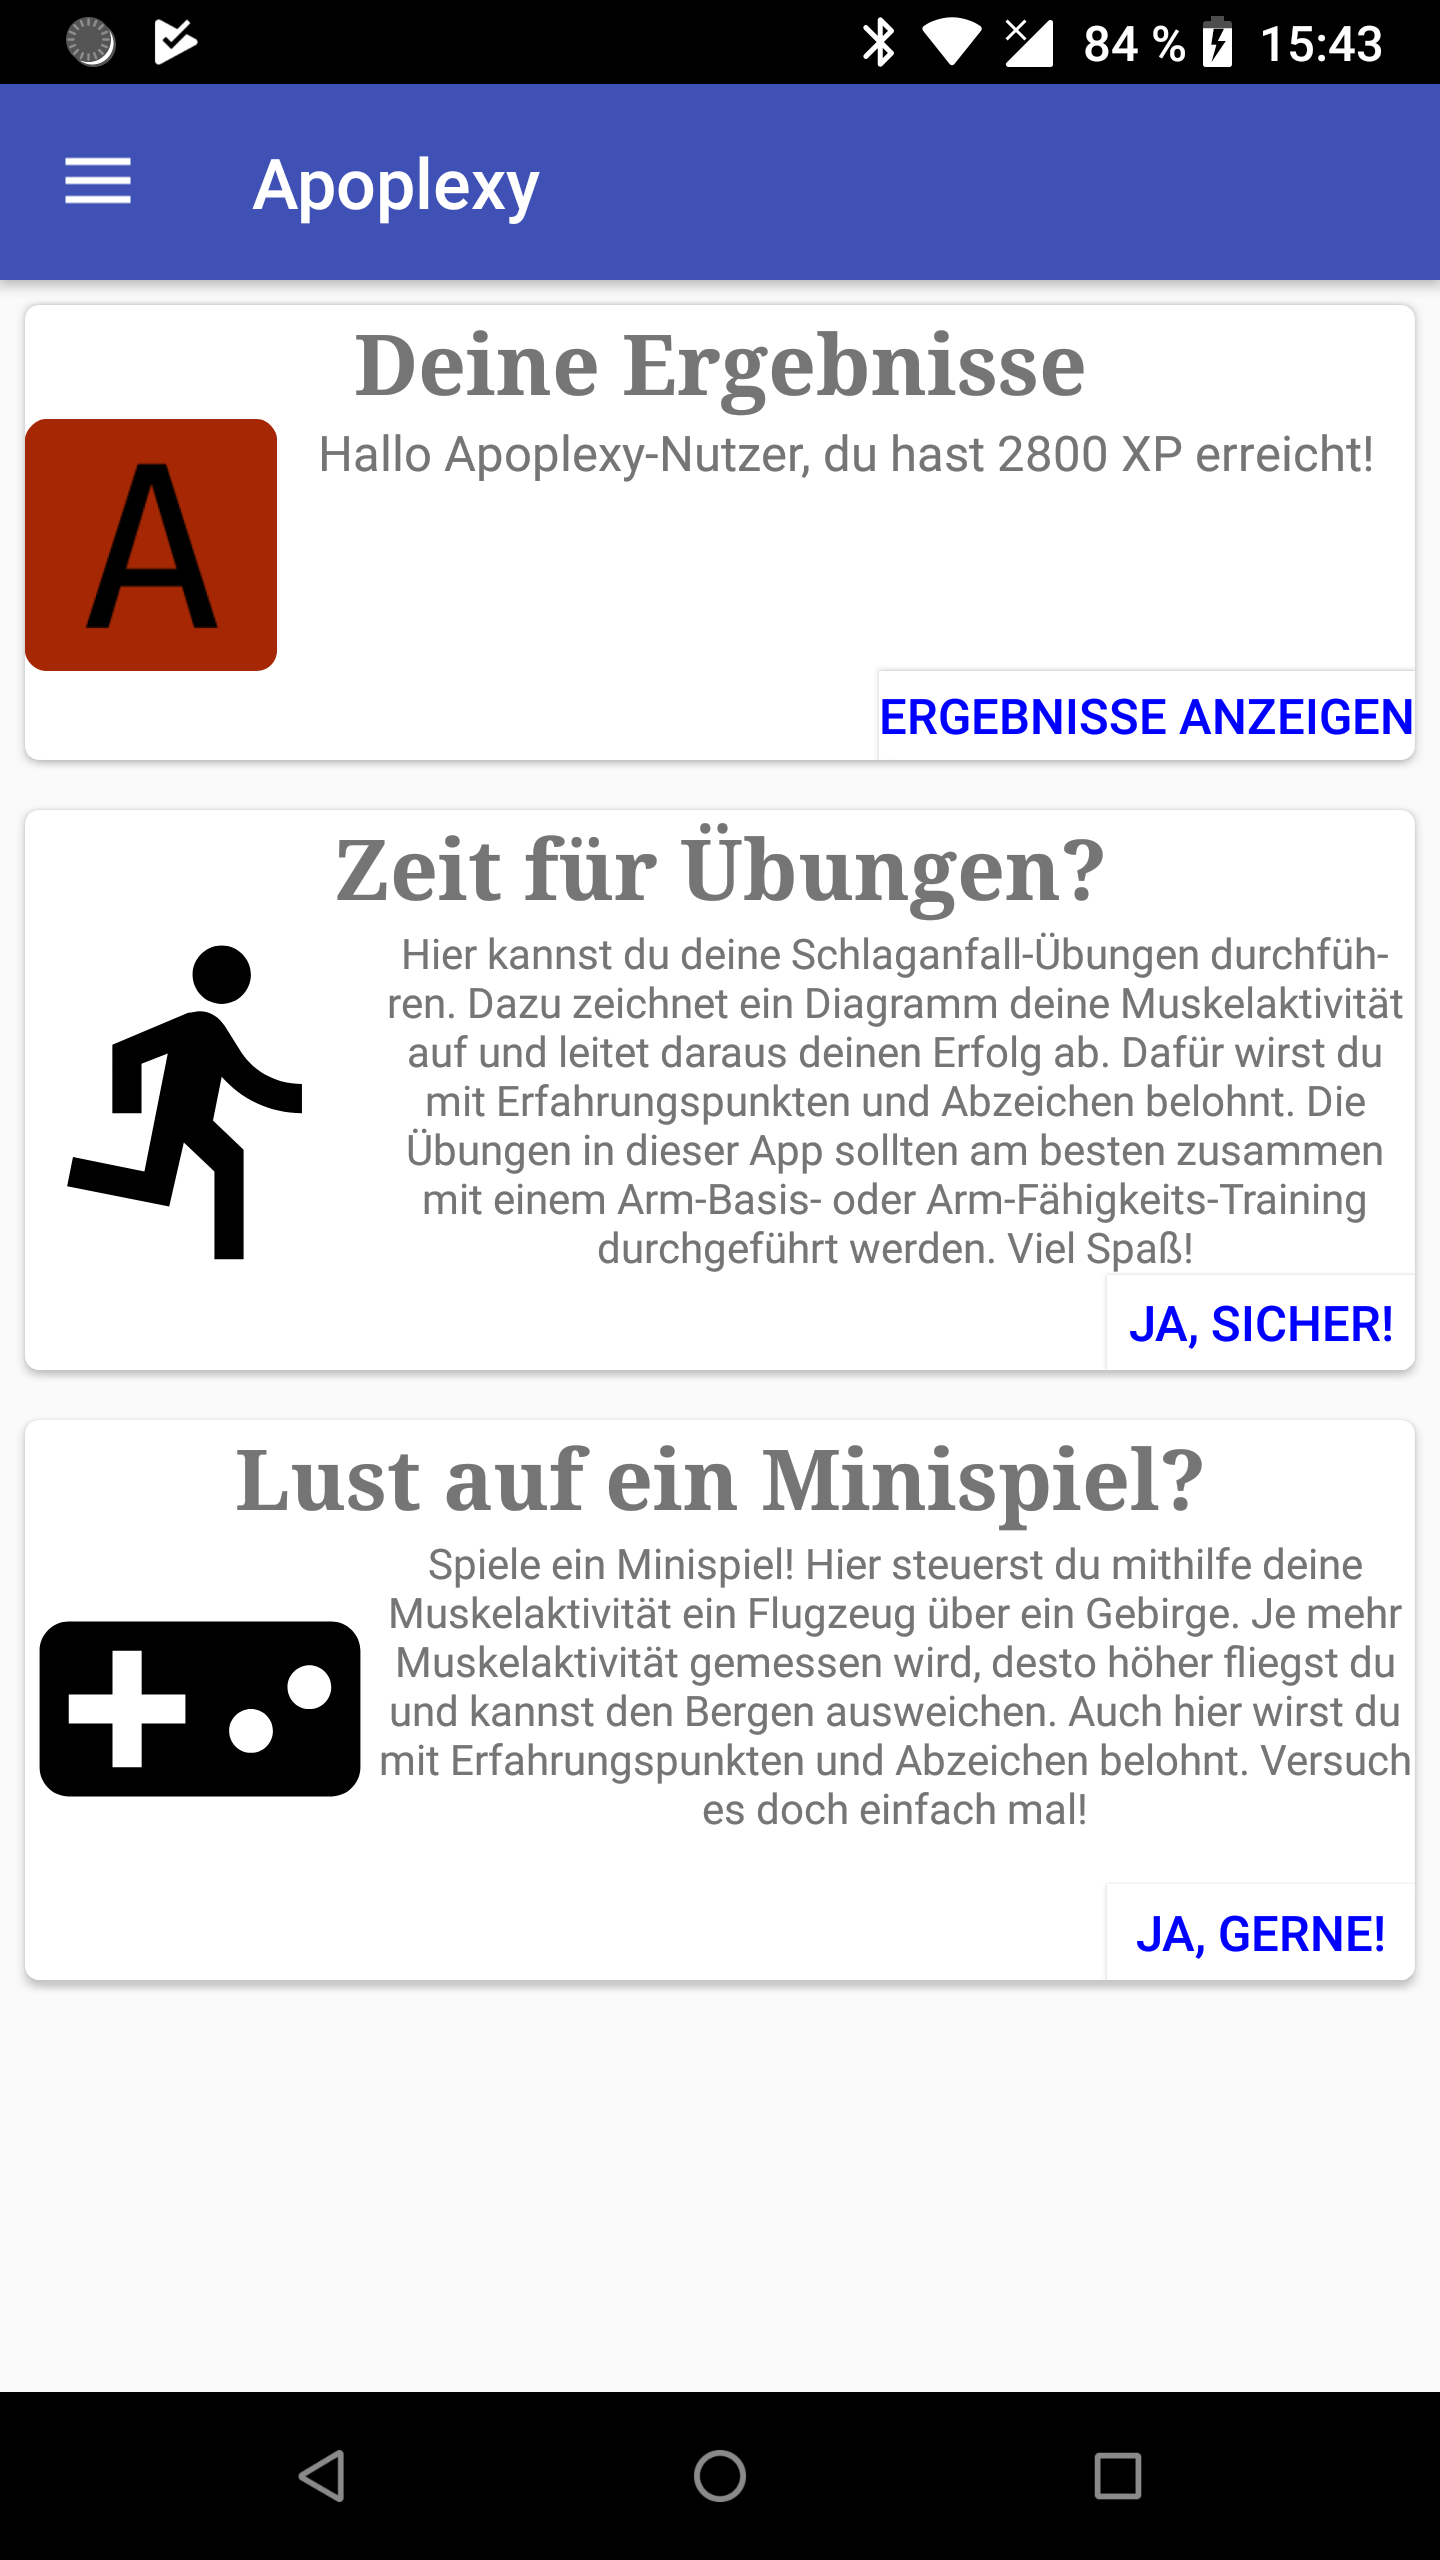
\includegraphics[width=0.6\colwidth]{pics/device-home}
   	\end{figure}
  \end{alertblock}

	\begin{alertblock}{Übungsseite der App}
		\begin{figure}[H]
			\centering
			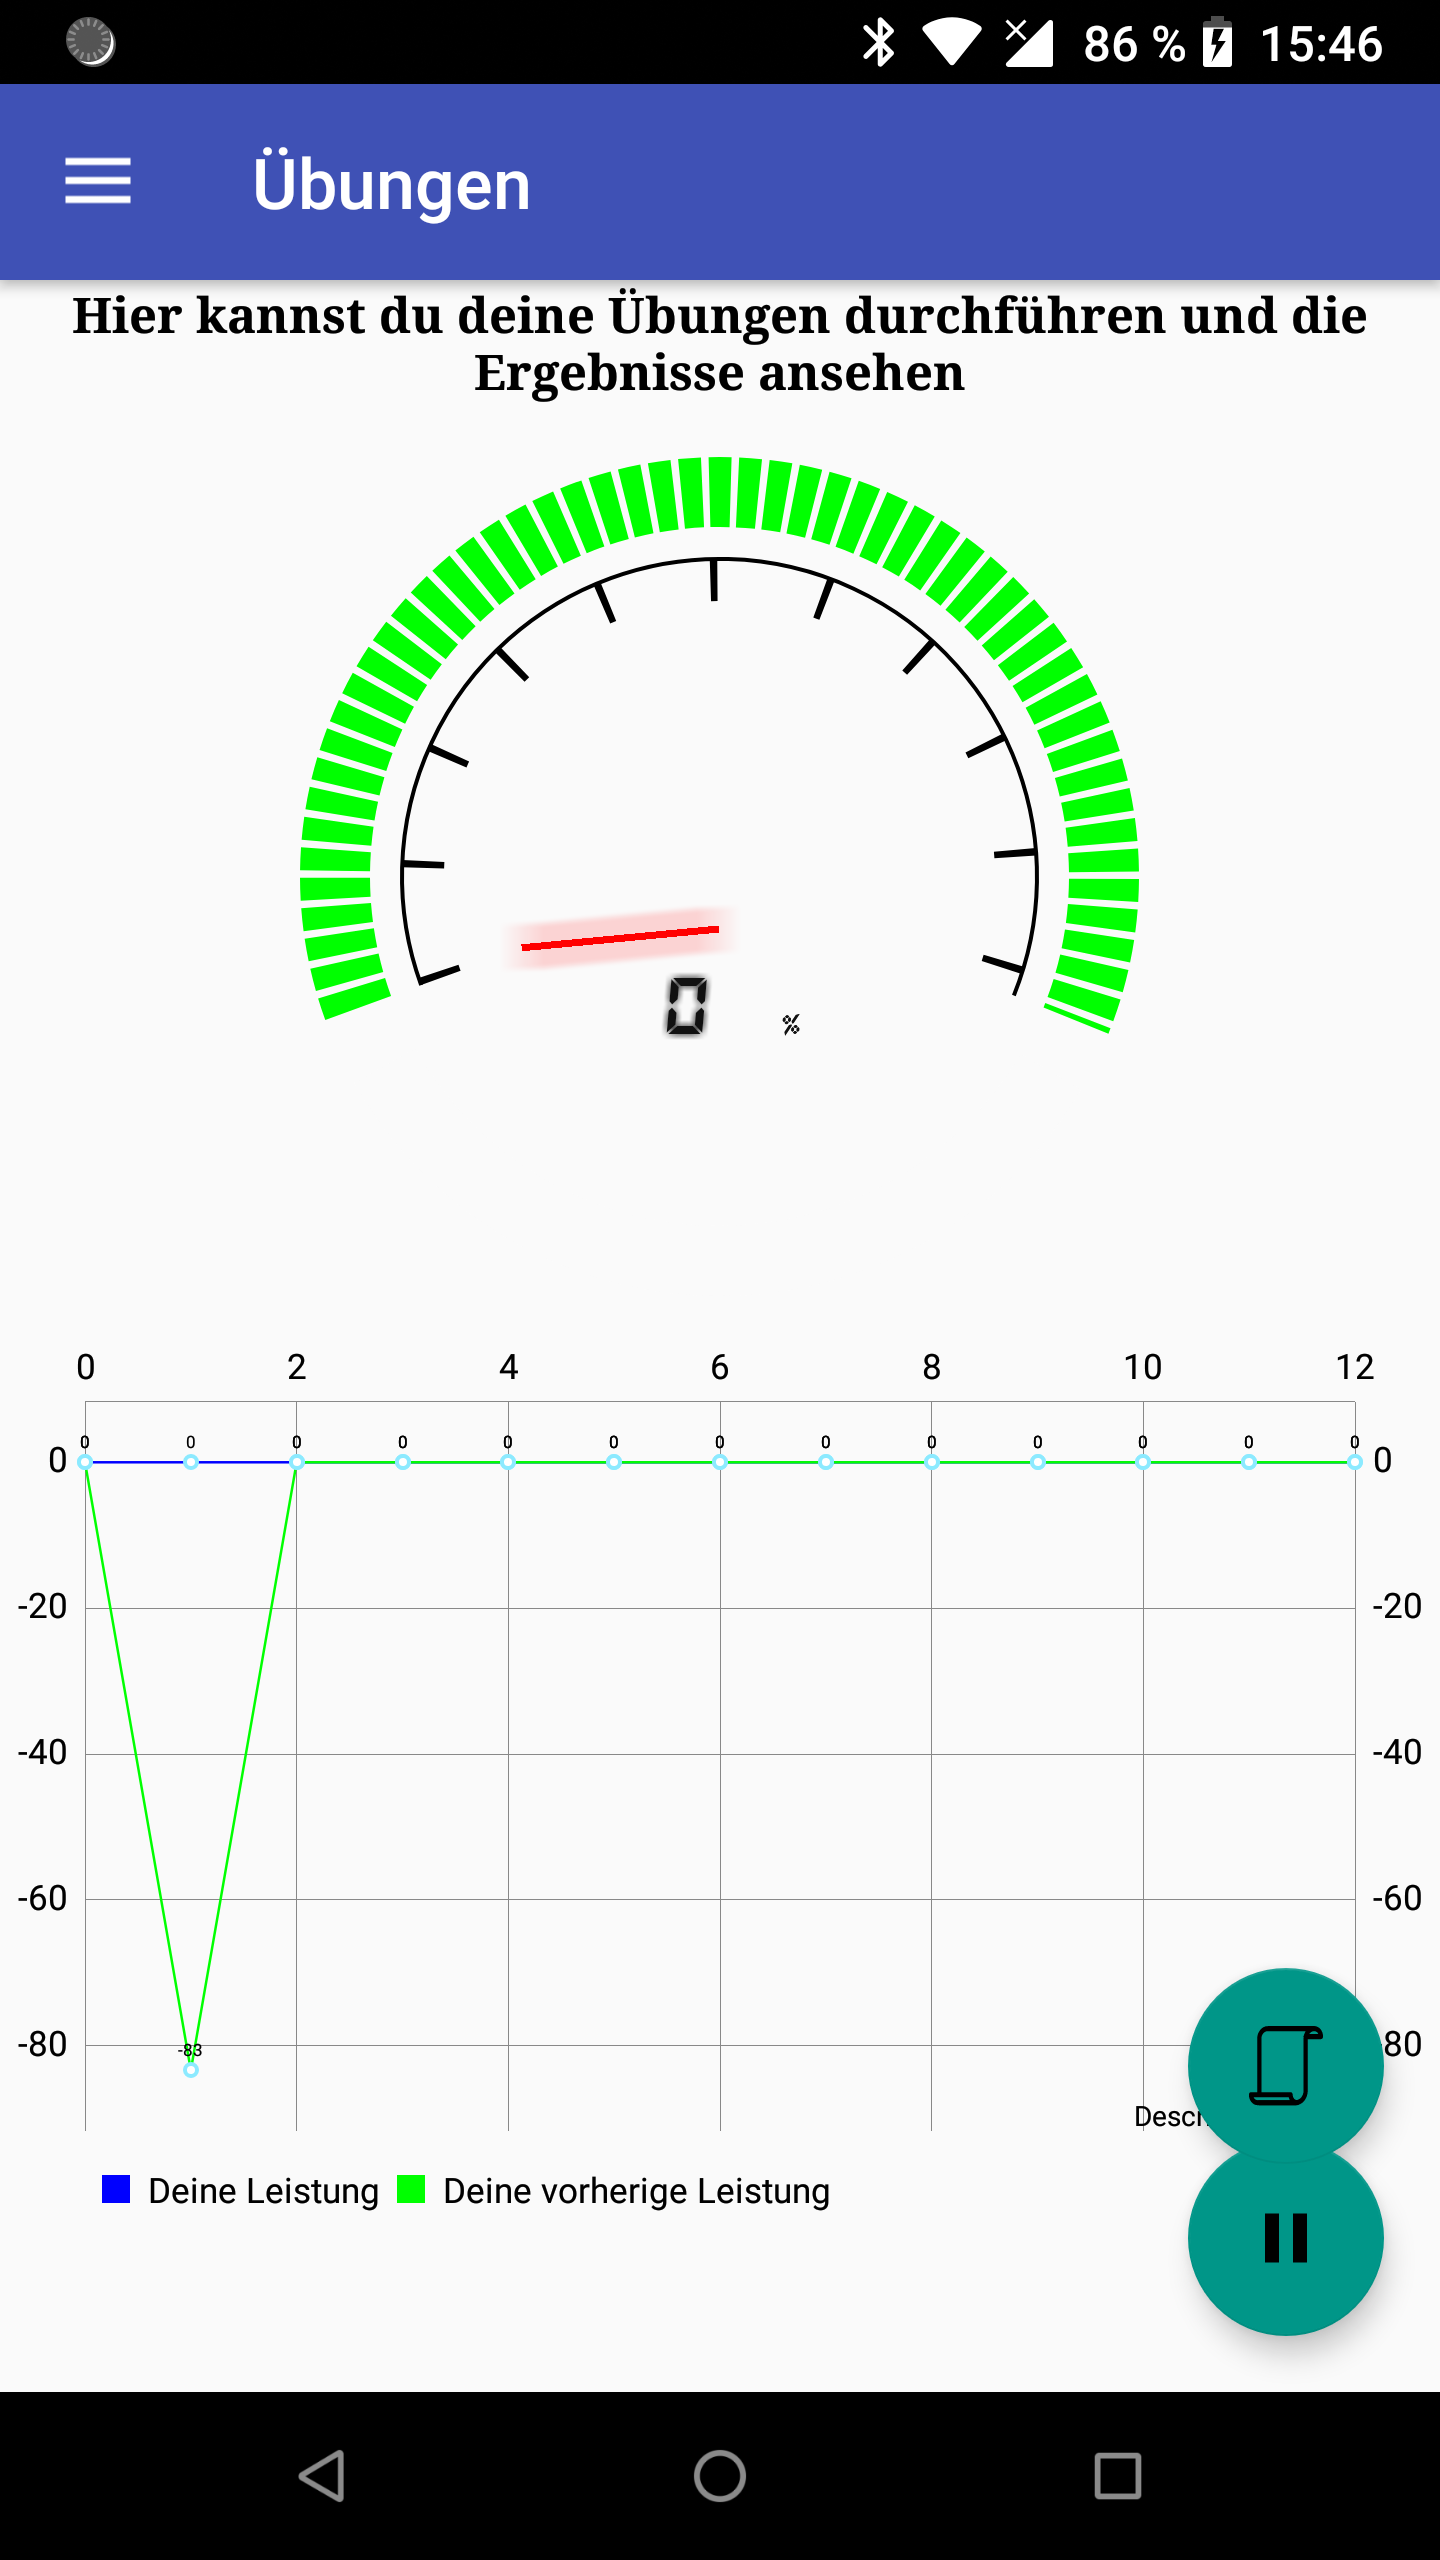
\includegraphics[width=0.6\colwidth]{pics/device-exercise}
		\end{figure}
	\end{alertblock}
\end{column}

\separatorcolumn
\begin{column}{\colwidth}  
	
	\begin{alertblock}{Das Minispiel}
		\begin{figure}[H]
			\centering
			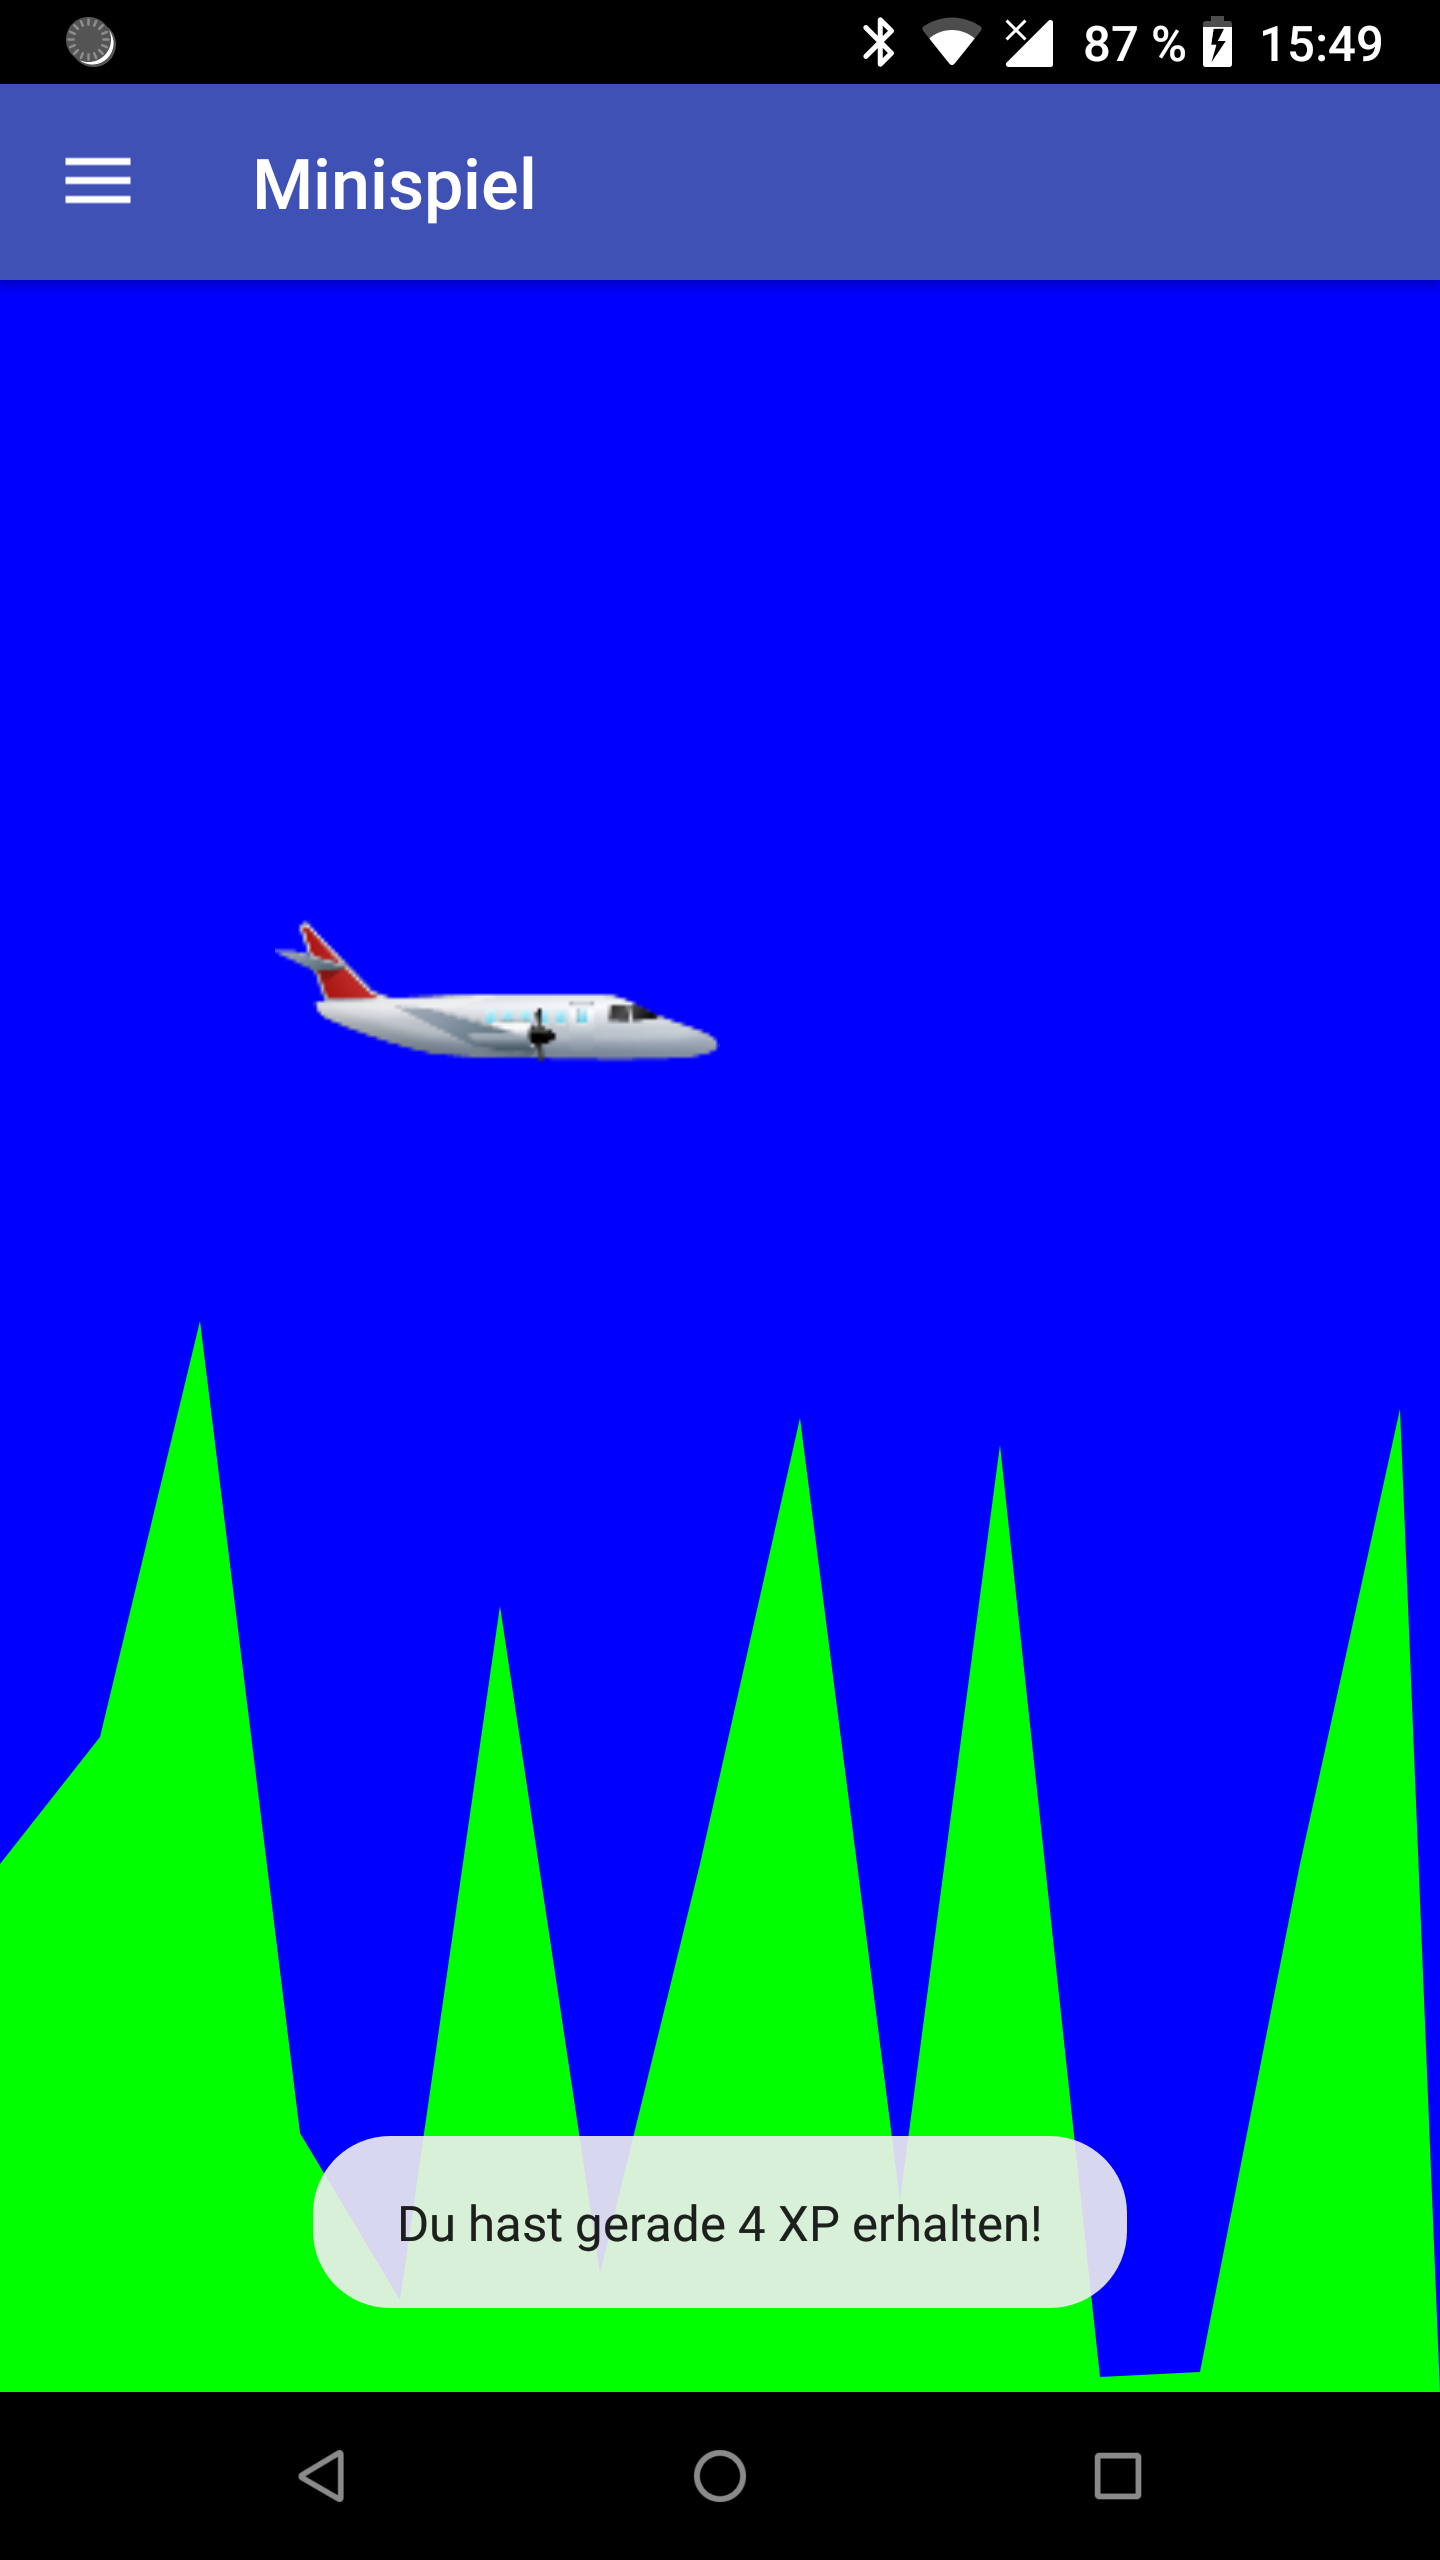
\includegraphics[width=0.6\colwidth]{pics/device-game}
		\end{figure}
	\end{alertblock}

	\begin{alertblock}{Anzeige der Quests}
		\begin{figure}[H]
			\centering
			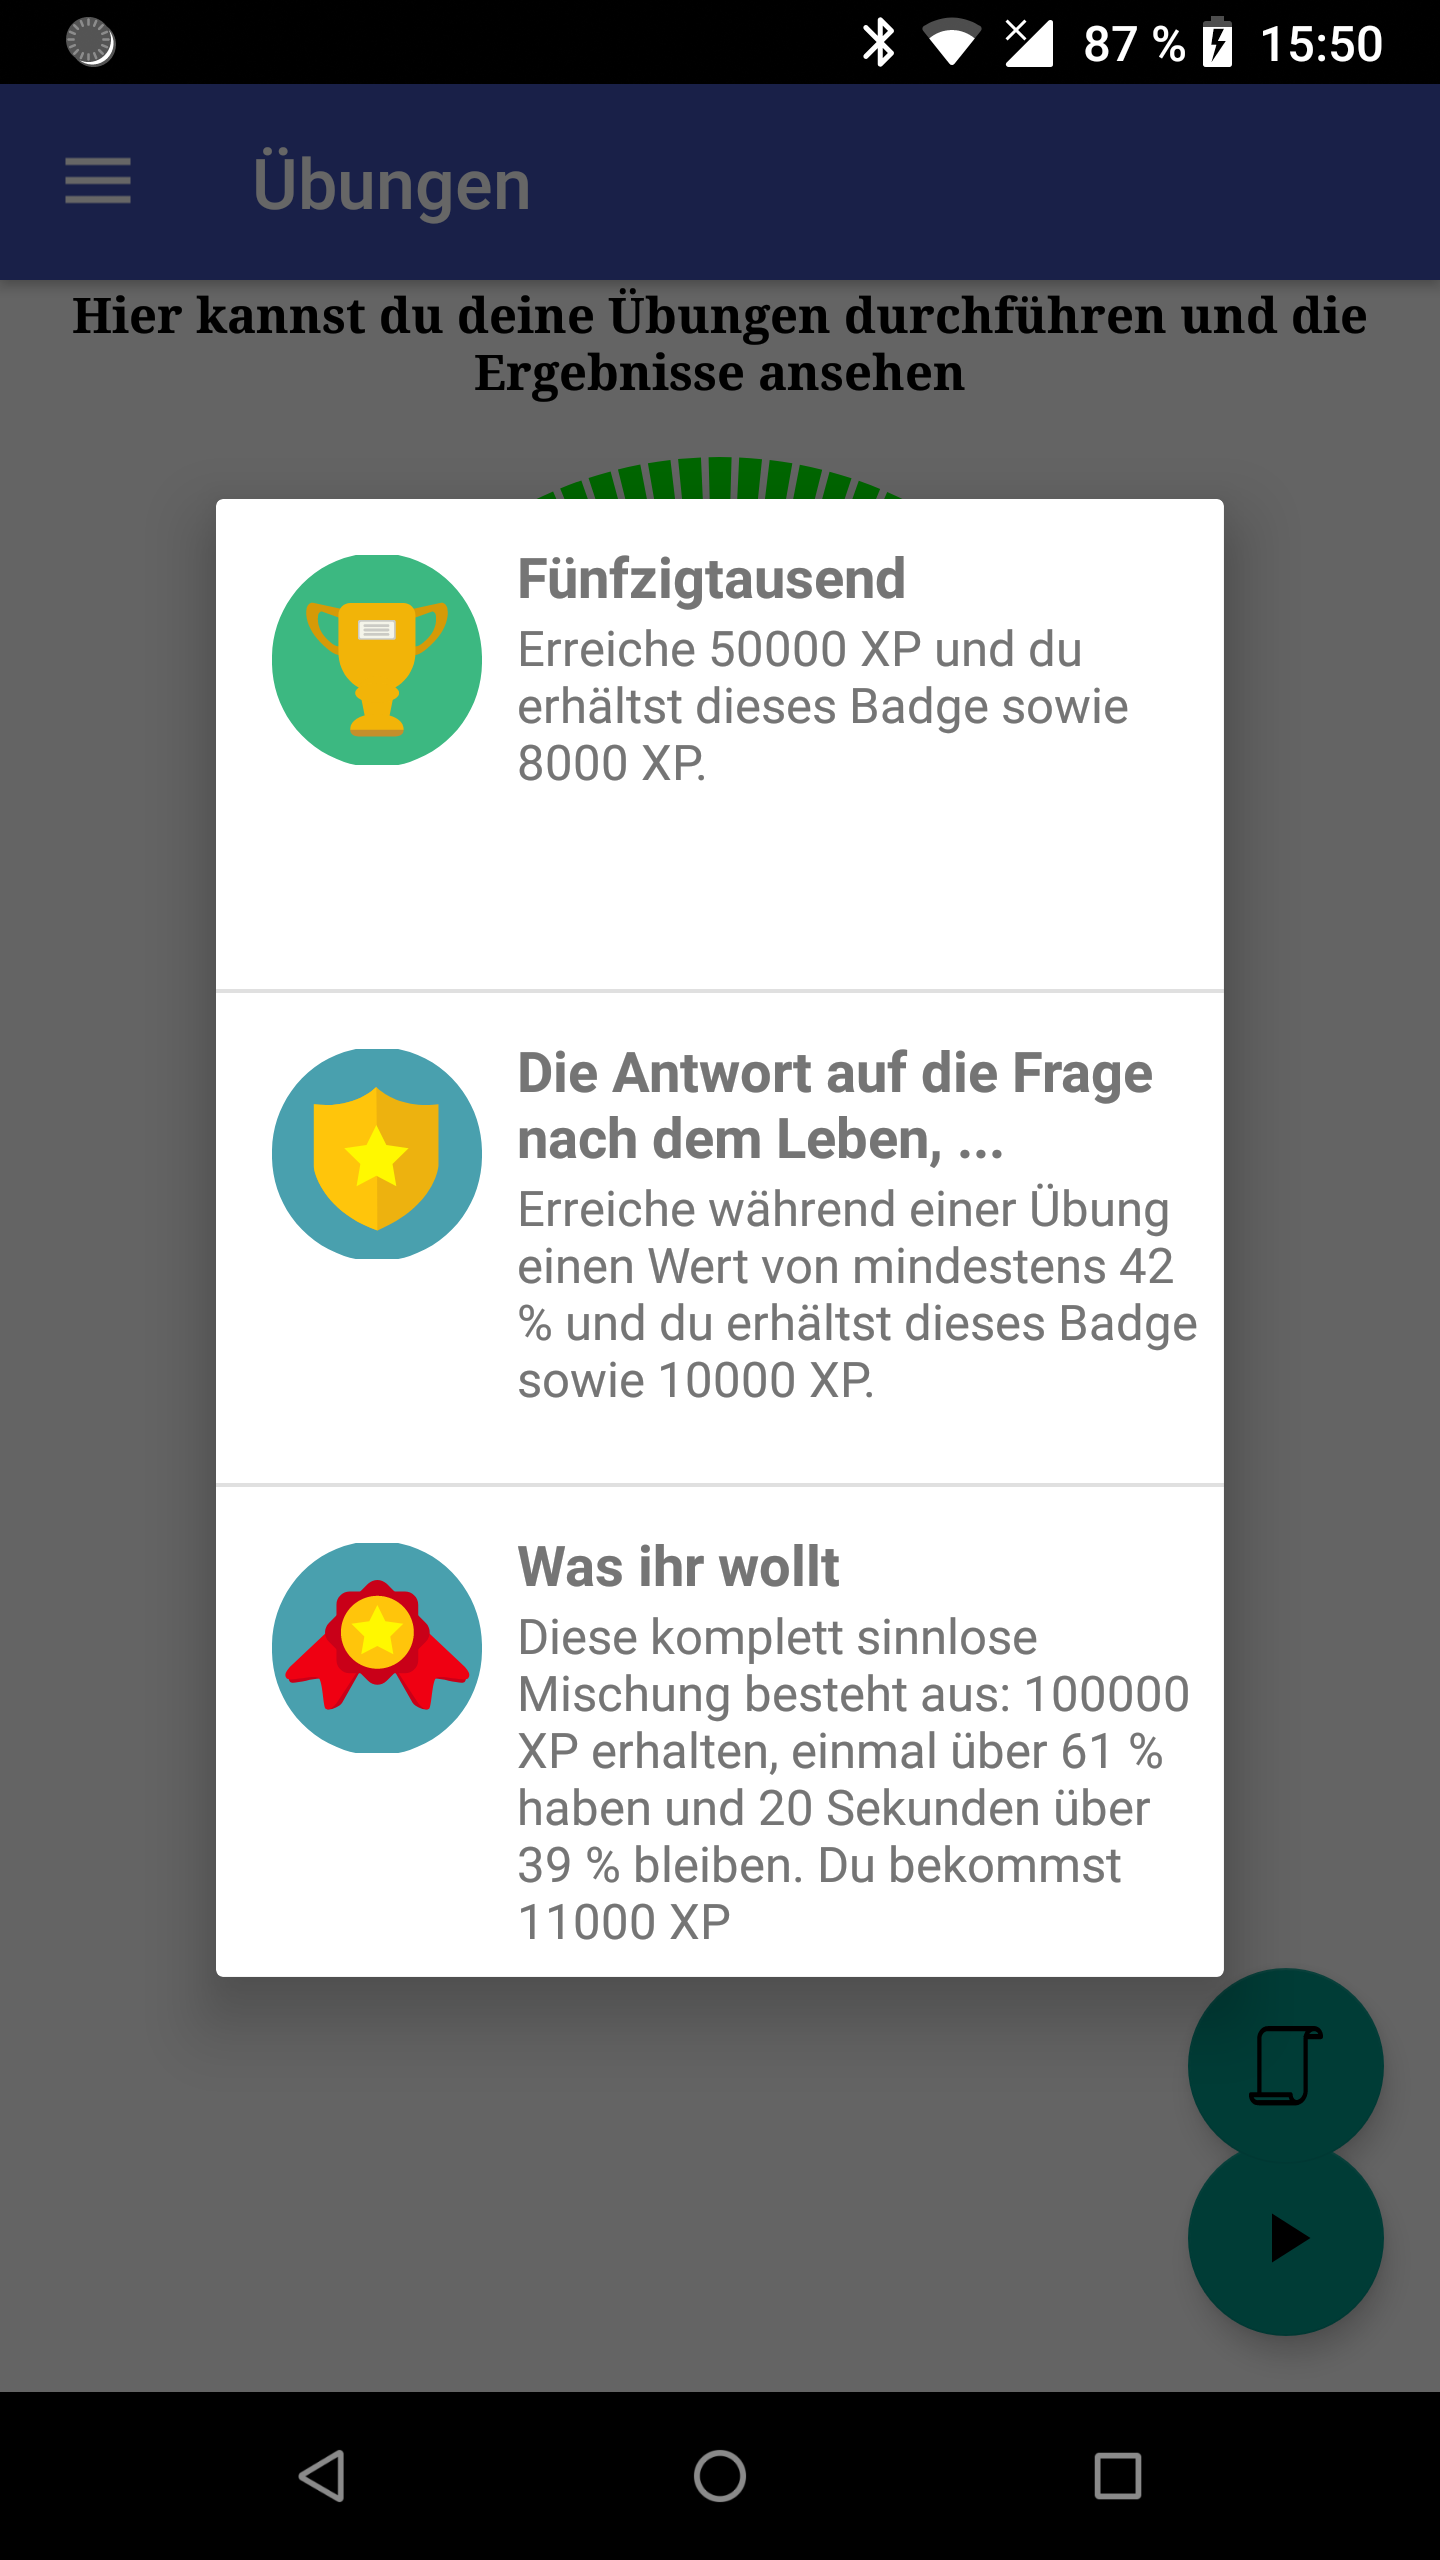
\includegraphics[width=0.6\colwidth]{pics/device-badges}
		\end{figure}
	\end{alertblock}

\end{column}

\separatorcolumn
\end{columns}
\end{frame}

\end{document}